\section{Test Reports}
\subsection{TR001: One Motor Test Rig}
\tr{T008}{AC008}{2}{BL012}{VPQ-21}
         {\shortstack[l]{GIVEN that we have a one motor test rig AND a microcontroller with a \\ working stabilizing code, WHEN we look at the test rig, THEN the \\motor  shall stay in the specified angle AND if we manually change angle; \\ the  motor shall adjust thrust accordingly.}}

\subsubsection*{\textsc{\medium Purpose}}
The purpose of TR001 is to gain information of how a single motor with a fixed pitch propeller can be stabilized in one axis. To conduct this test, and fulfil AC008, a motor is mounted on an arm that can alter position in one axis. 

\subsubsection*{\textsc{\medium Test Setup}}
In Tab. \ref{tab:tabt1} the equipment used conducting TR001 is displayed. 
\begin {table}[H]
    \begin{center}
    \caption {Test Equipment: One Motor Test Rig} 
    \label{tab:tabt1} 
    \begin{tabular}{|l|l|l|}\hline 
        Brushless motor    & DJI E800   &\\ \hline
        ESC         & DJI E620S     &\\ \hline
        Power Supply & EA-PS 2342-06 B  & 20 V   \\ \hline
        Microcontoller & Arduino Nano ATmega328P &\\ \hline
        IMU & MPU5060 & \\ \hline
    \end{tabular}
    \end{center}
\end{table}

\noindent
In Fig. \ref{fig:onemotor} an illustration of the test setup for the One Motor Test Rig is displayed. The DJI E800 motor is mounted on an arm that can variate position in one axis. 

\begin{figure}[H]
    \centering
    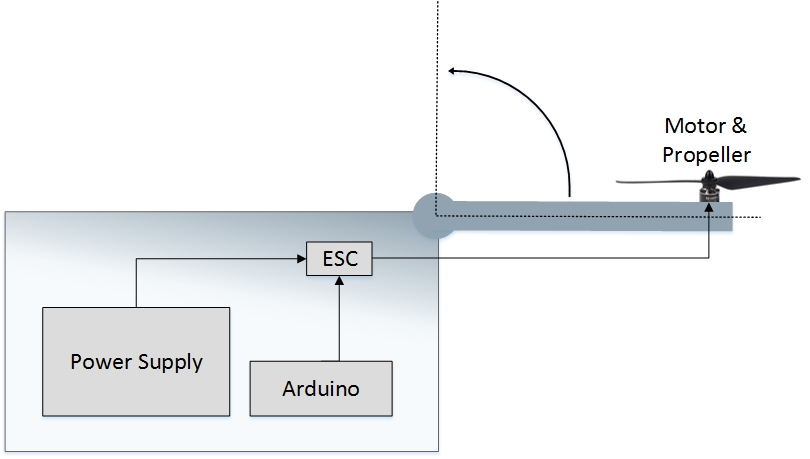
\includegraphics[width = 0.8\textwidth]{VAPIQ-PICTURES/TestSetup1}
    \caption{Test Setup: One Motor Test Rig}
    \label{fig:onemotor}
\end{figure}

\noindent On the arm the MPU5060 is mounted, and this sensor transmits position data to the Arduino Nano. The Arduino Nano will then transmit a PWM signal to the ESC that equals desired thrust to the motor based on the measured sensor value. The amount of thrust is determined by the current position relative to desired position. 
\\\\
In Appendix A1 the code used for the One Motor Test Rig is displayed. For this test we used the $PID\_v1.h$ library to control and stabilize the arm. Before conducting this test we determined the most appropriate PID parameters by trial and error. These parameters are displayed in Tab. \ref{tab:tabt2}.
\begin {table}[H]
    \begin{center}
    \caption {PID Parameters: One Motor Test Rig} 
    \label{tab:tabt2} 
    \begin{tabular}{|l|l|}\hline 
        Kp         & 5  \\ \hline
        Ki         & 2   \\ \hline
        Kd         & 1  \\ \hline
    \end{tabular}
    \end{center}
\end{table}

\subsubsection*{\textsc{\medium Test Summary}}
\noindent
In code the desired angle (Setpoint = desired angle;) was set before transferring code to the microcontroller. When a desired angle was implemented and the code was compiled and transferred; the motor provided the appropriate thrust and the the motor arm moved to the wanted position. 
\\\\
When the arm was manually moved in a positive or negative direction relative to the desired angle the motor produced less or more thrust as intended.

\subsubsection*{\textsc{\medium Test Assessment}}
% [Enter a comprehensive assessment of your interpretation of how adequate the test was in light of how thorough the test plan said it should be? What wasn't tested well enough?]
%[Describe any variances between the testing that was planned and the testing that actually occurred.  Also, provide an assessment of the manner in which the test environment may be different from the operational environment and the effect of this difference on the test results
%[Provide a brief description of the unexpected results, problems, or defects that occurred during the testing.]
When using using libraries it is difficult to have an overview of how the code functions, unless the libraries are self composed. This may be a source of error.
\\\\
In this test, there were some measurement inaccuracy concerning the actual angle of the test arm and the angle input. This is due to the fact that there was no device measuring the actual arm angle. Also sensor instability was a reoccurring problem during the tests. Calibration and filtering of noise had to be done in order to achieve more stable results, and it still have potential for improvements.
\\\\

\subsubsection*{\textsc{\medium Test Results}}
In this test the arm stayed in approximately the desired angle. In Tab. \ref{tab:tabt3} the results of the One Motor Test Rig is displayed. 
\begin {table}[H]
    \begin{center}
    \caption {Test Results: One Motor Test Rig} 
    \label{tab:tabt3} 
    \begin{tabular}{|l|l|l|}\hline 
        Test No.:  & Desired Angle:   & Comment:\\ \hline
        1         & 45    &  Arm stabilizes   \\ \hline
        2         & 30    &  Arm stabilizes    \\ \hline
        3         & 10    &  Arm stabilizes    \\ \hline
    \end{tabular}
    \end{center}
\end{table}
\newpage

%%%%%%%%%%%%%%%%%%%%%%%%%%%%%%%%%%%%%%

\subsection{TR002: Arduino Nano Computation Time}
\tr{T010}{AC013}{3}{BL033}{VPQ-106 VPQ-107}
         {\shortstack[l]{GIVEN that we have an Arduino Nano, WHEN we run a script,THEN \\the microcontroller shall complete all computations within 20 ms.}}
                         
\subsubsection*{\textsc{\medium Purpose}}
The purpose of TR002 is to determine if we can use an Arduino Nano as an on-board chip for our quadcopter. We will measure the time it takes for the control loops to compute. It is expected that the computation time is between 1 ms to 5 ms. 

\subsubsection*{\textsc{\medium Test Setup}}
In Tab. \ref{tab:tabt4} the equipment used conducting TR002 is displayed. 
\begin {table}[H]
    \begin{center}
    \caption {Test Equipment: Arduino Nano Computation Time} 
    \label{tab:tabt4} 
    \begin{tabular}{|l|l|}\hline 
        Power Supply & EA-PS 2342-06 B     \\ \hline
        Microcontoller & Arduino Nano ATmega328P \\ \hline
        IMU & MPU5060 \\ \hline
        LED & \\ \hline
        Oscilloscope & \\ \hline
        \end{tabular}
    \end{center}
\end{table}

\noindent A flight controller normally have two loops; one for attitude control and one for rate control. Both these loops needs to be completed within 20ms. Having an unequipped on-board chip can put restrictions on the stabilization of the quadcopter. The test is conducted by running a loop and at the beginning of the loop a LED is set high, and at the end of the loop, low. To measure the computation time; an oscilloscopes measuring probe was connected to the LED. 

\subsubsection*{\textsc{\medium Test Assessment}}
At this point in the project the size of the code is assumed to be smaller than it will be in the future. 

\subsubsection*{\textsc{\medium Test Results}}
In Tab. \ref{tab:tabt5} the time needed for the Arduino Nano to carry out its computations are displayed.  
\begin {table}[H]
    \begin{center}
    \caption {Test Results: Arduino Nano Computation Time} 
    \label{tab:tabt5} 
    \begin{tabular}{|c|c|}\hline 
        Test No.: &  Result [ms]:\\ \hline
        1. & 1.66 \\ \hline
        2. & 1.81 \\ \hline
        3. & 1.79 \\ \hline
    \end{tabular}
    \end{center}
\end{table}
\noindent
The Arduino Nano Computation time turned out to be around the expected value. The worst case computation time was $1.81ms$ as shown in \ref{tab:tabt5}. 

\newpage

%%%%%%%%%%%%%%%%%%%%%%%%%%%%%%%%%%%%%%

\subsection{TR003: 1-Axis Stabilization FPQ}
\tr{T011}{AC014}{3, 4}{BL033, BL032}{VPQ-106, VPQ-107}
         {\shortstack[l]{GIVEN that we have a one axis test rig AND a microcontroller with a \\working
                         stabilization code, WHEN we look at the test rig AND the code\\ is running,
                         THEN the one axis test rig shall stay in the specified angle \\AND if the 
                         angle is manually changed; the motors shall adjust thrust\\ accordingly.}}
                         

\subsubsection*{\textsc{\medium Purpose}}
The purpose of TR003 is to gain information of how to obtain stability, how to tune a controller and test sensors and their output. To do this, two motors with fixed pitch propellers are tested in 1-axis. To conduct this test, and fulfil AC014, one motor is mounted on each side of the testing rig which pivots around its center allowing movement in 1-axis. 

\subsubsection*{\textsc{\medium Test Setup}}
In Fig. \ref{fig:testsetup3} an illustration of the test setup for the 1-axis test rig is displayed. 
\begin{figure}[H]
    \centering
    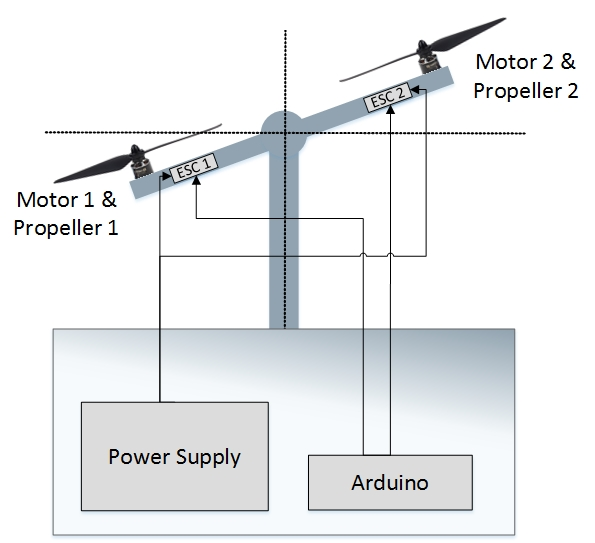
\includegraphics[width = 0.5\textwidth]{VAPIQ-PICTURES/TestSetup3}
    \caption{Test Setup: 1-Axis Test Rig}
    \label{fig:testsetup3}
\end{figure}

\noindent This test has been conducted in many iterations. It has been done with multiple sensors and multiple versions of code. On the test rig an IMU is mounted, and this sensor transmits position data to the Arduino Nano. The Arduino Nano will then transmit a PWM signal to the ESC that equals desired thrust to the motors based on the measured sensor values. The amount of thrust is determined by the current position relative to desired position. To stabilize the test rig a self-developed P-control has been implemented. \\
\\
In Appendix A2 the current code for TR003 can be found.

\subsubsection*{\textsc{\medium Test Summary}}
%[Include basic information about what was tested and what happened.]
All testing performed on the 1-axis test rig has been done to understand and document how the stabilization algorithms and sensors are performing. The 1-axis rig has been used continuously for testing stability, sensors and code for fixed pitch. 

\subsubsection*{\textsc{\medium Test Assessment}}
% [Enter a comprehensive assessment of your interpretation of how adequate the test was in light of how thorough the test plan said it should be? What wasn't tested well enough?]
%[Describe any variances between the testing that was planned and the testing that actually occurred.  Also, provide an assessment of the manner in which the test environment may be different from the operational environment and the effect of this difference on the test results
%[Provide a brief description of the unexpected results, problems, or defects that occurred during the testing.]
During testing there has been problems with sensor instability when propellers have been mounted. This was a reoccurring problem with all sensors. Calibration and filtering of noise had to be done in order to achieve more stable results.

\subsubsection*{\textsc{\medium Test Results}}
The results obtained when conducting tests on this test rig has been valuable. We have gained information about the construction of a flight controller, stabilization algorithms and implementation of sensors continuously throughout the project.\\
\\
See code in Appendix A2.
\newpage

%%%%%%%%%%%%%%%%%%%%%%%%%%%%%%%%%%%%%%

\subsection{TR004: FPQ Hover Stabilization}
\tr{T012}{AC015}{4}{BL035 BL036}{VPQ-178 VPQ-184}
         {\shortstack[l]{GIVEN that we have assembled a FPQ, WHEN it is secured on \\ test table AND we let the FPQ hover, THEN it shall stabilize itself.}}
\subsubsection*{\textsc{\medium Purpose}}
%hvorfor gjør vi dette?
The purpose of TR004 is to see how stable the quadcopter is in hover.

\subsubsection*{\textsc{\medium Test Setup}}
% hvordan gjør vi dette?
Fig. \ref{fig:ft1} and \ref{fig:ft2} shows the quadcopter secured on test table.

\begin{figure}[h]
        \centering
         \begin{minipage}[b]{0.495\textwidth}
            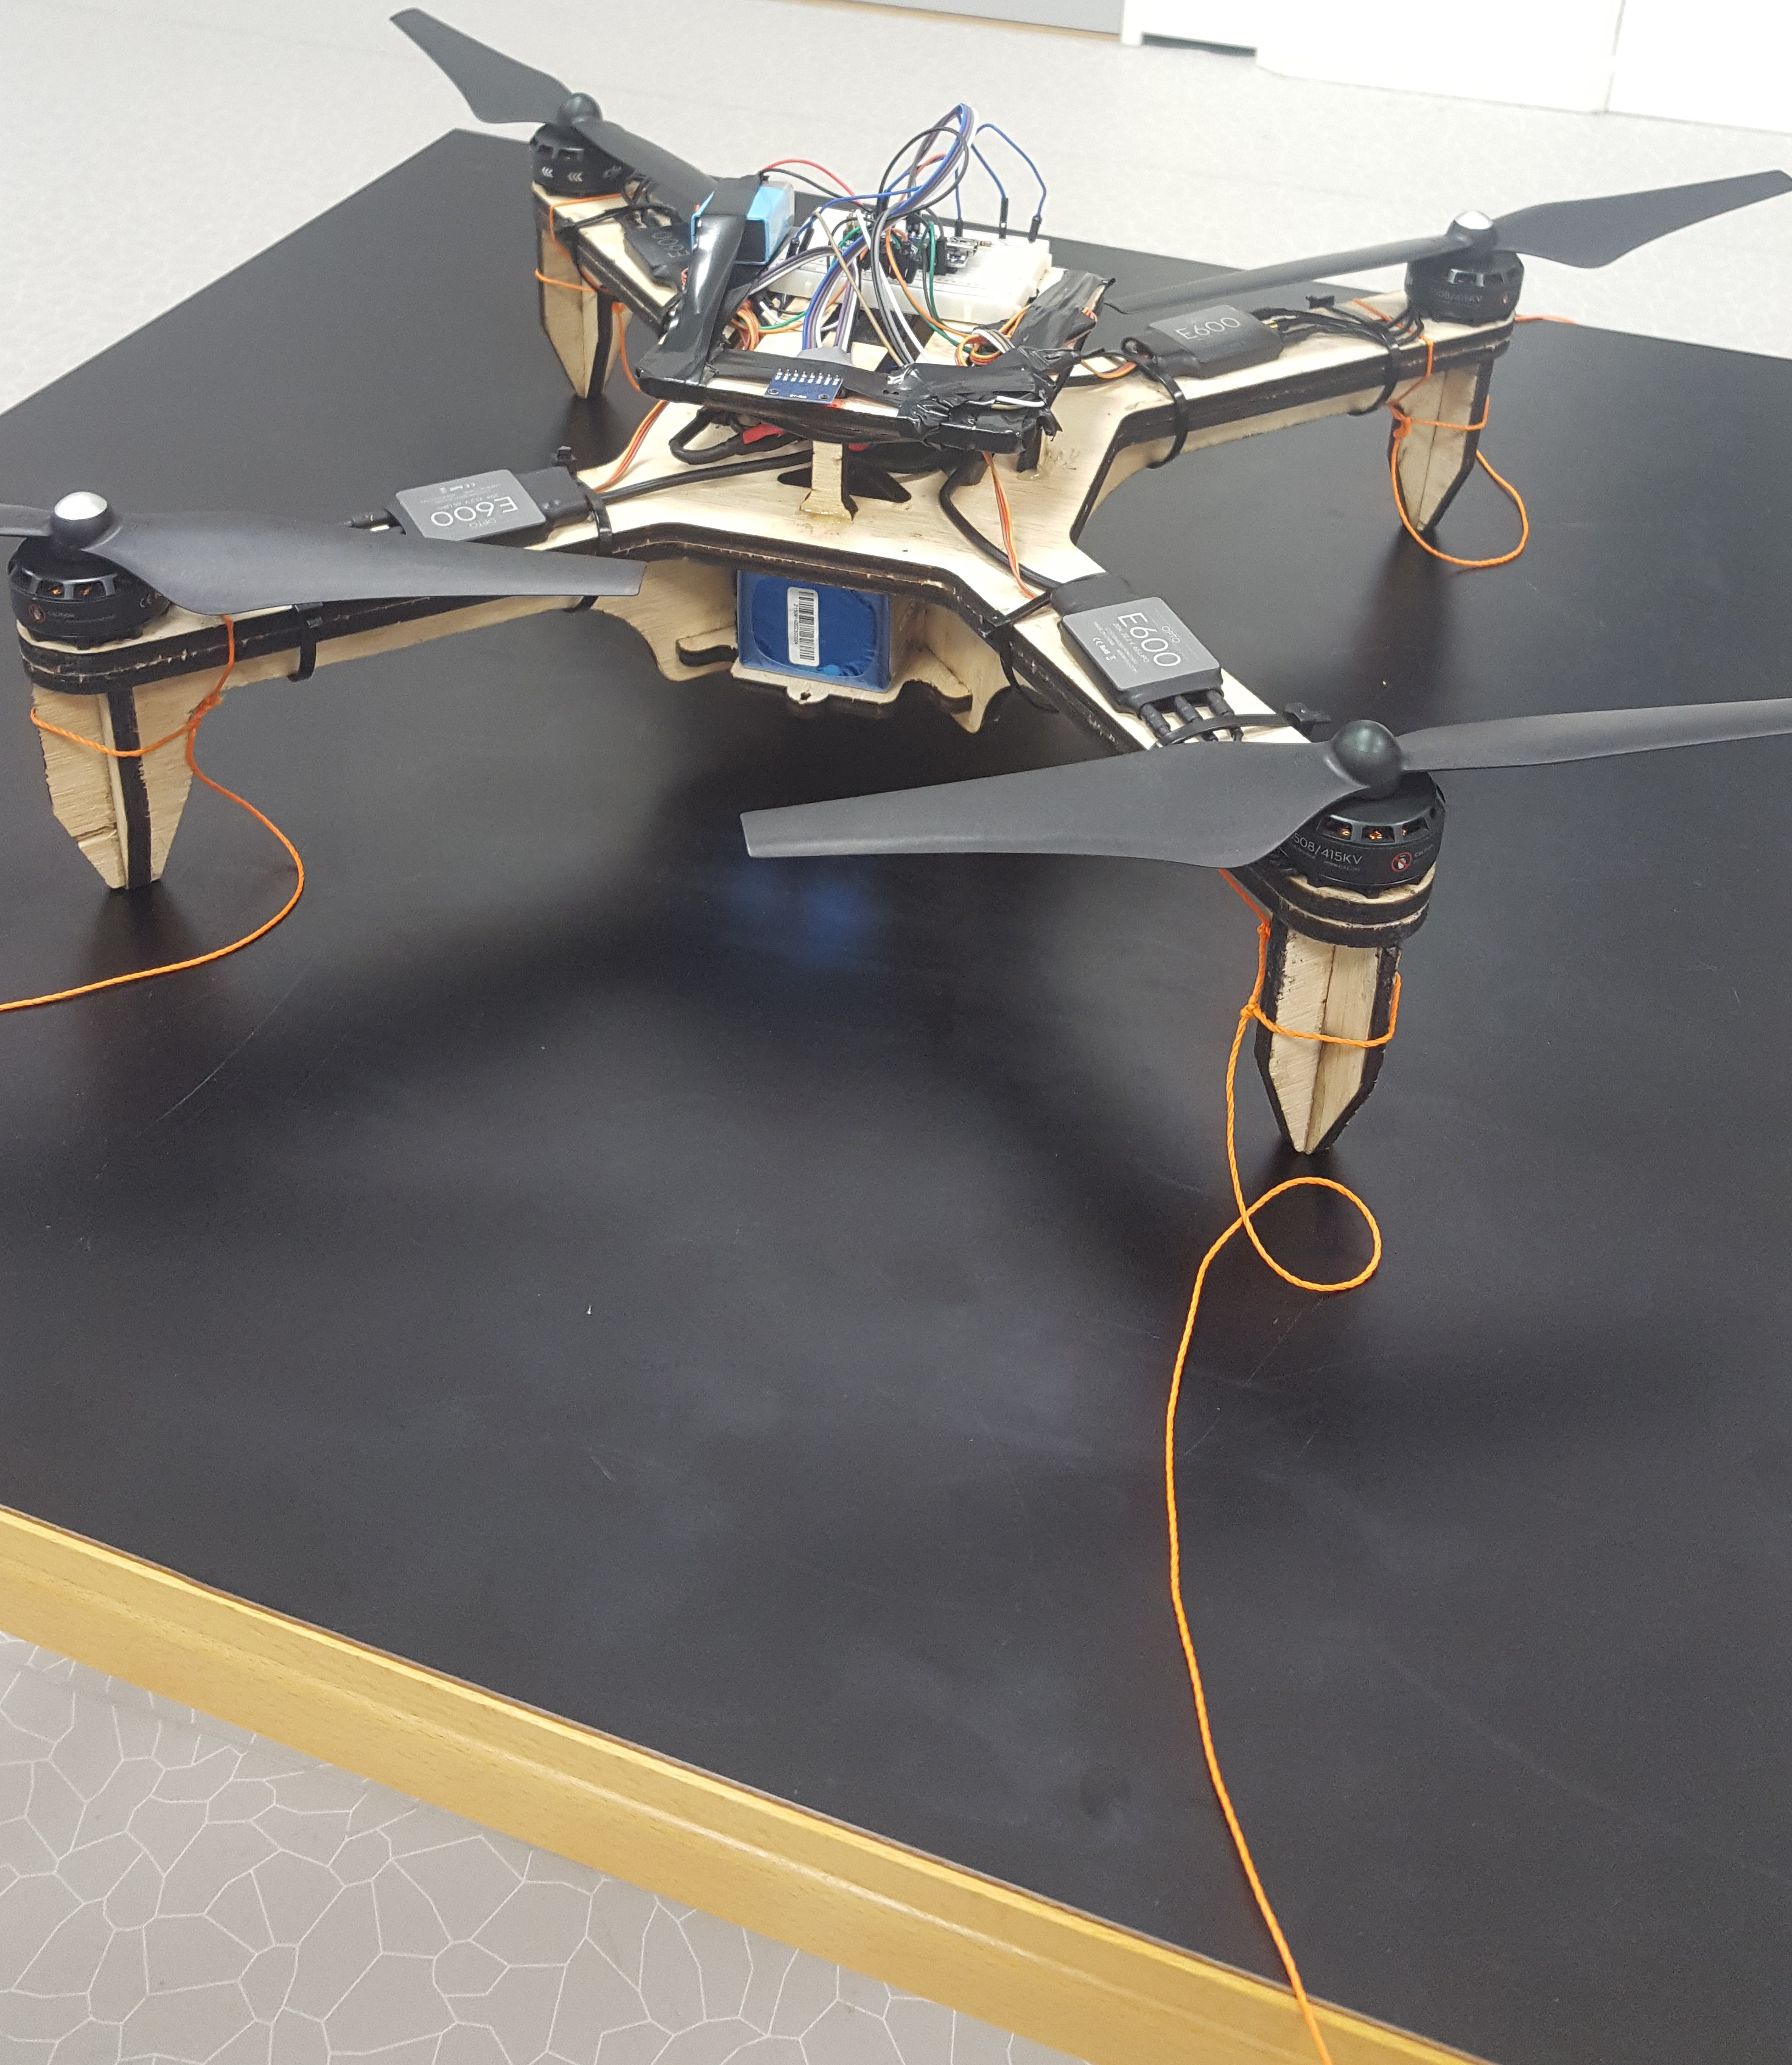
\includegraphics[width = 1\textwidth]{VAPIQ-PICTURES/flighttest2}
            \caption{Test Setup: Quadcopter Tied to Test Table}
            \label{fig:ft1}
        \end{minipage}
        \hfill
        \begin{minipage}[b]{0.45\textwidth}
            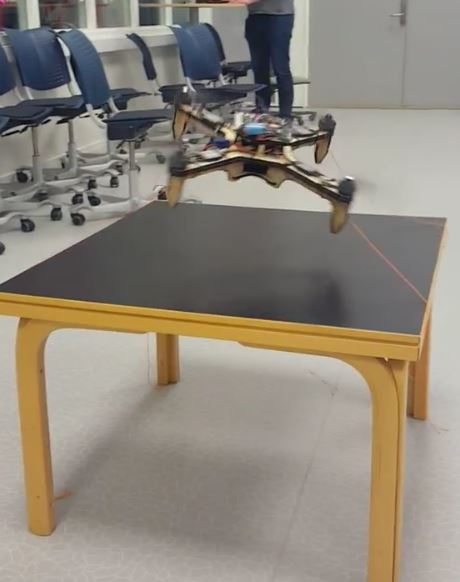
\includegraphics[width = 1\textwidth]{VAPIQ-PICTURES/flighttest}
            \caption{Quadcopter in Flight}
            \label{fig:ft2}
        \end{minipage}
\end{figure}

\noindent In this test the stability of the quadcopter at hover is tested. The quadcopter was secured to a table by threads on each leg, ensuring that it could not uncontrollably fly away. In Appendix A4 the code used for TR004 can be found. 

\subsubsection*{\textsc{\medium Test Assessment}}
% egenvurdering av testen
% [Enter a comprehensive assessment of your interpretation of how adequate the test was in light of how thorough the test plan said it should be? What wasn't tested well enough?]

%[Describe any variances between the testing that was planned and the testing that actually occurred.  Also, provide an assessment of the manner in which the test environment may be different from the operational environment and the effect of this difference on the test results
%[Provide a brief description of the unexpected results, problems, or defects that occurred during the testing.]
The quadcopter was very unstable. The reason for this might be noise on sensor. Another factor may be when the quadcopter hits the end of the line a reaction force is experienced by the quadcopter, telling the sensors that a dramatic change in position has occurred, thus making the quadcopter overcompensate and react unstable. 
\\\\
At this point it can be concluded that a combination of these factors are the reason for unstable flight.

\subsubsection*{\textsc{\medium Test Results}}
%hva fikk vi ut av dette
The quadcopter hovers, but did not stabilize. See video included on USB.
\newpage
%%%%%%%%%%%%%%%%%%%%%%%%%%%%%%%%%%%%%%

\subsection{TR005: Motor Propeller Thrust Test Rig}
\tr{T013}{AC016}{4}{BL037}{VPQ-184}
         {\shortstack[l]{GIVEN that we have a test rig for testing motor and propeller\\ combinations AND a code where we can manually alter thrust, WHEN \\we alter thrust, THEN the weight will display thrust in grams.}}

\subsubsection*{\textsc{\medium Purpose}}
The purpose of TR005 is to evaluate the performance of the different motor and propeller combinations for fixed pitch. 

\subsubsection*{\textsc{\medium Test Setup}}
In Tab. \ref{tab:tabt6} and \ref{tab:tabt7} the equipment used conducting TR005 is displayed.
\begin {table}[H]
    \begin{center}
    \caption {Test Equipment: Motor Propeller Thrust Test Rig} 
    \label{tab:tabt6} 
    \begin{tabular}{|l|}\hline 
        Power SupplyEA-PS 2342-06 B           \\ \hline
        Microcontoller Arduino Nano ATmega328P \\ \hline
        Motor \\ \hline
        ESC\\ \hline    
        \end{tabular}
    \end{center}
\end{table}

\begin {table}[H]
    \begin{center}
    \caption {Motor Propeller Combination: Motor Propeller Thrust Test Rig} 
    \label{tab:tabt7} 
    \begin{tabular}{|l|l|}\hline 
        Motor Test No. 1: & Motor Test No. 2:    \\ \hline
        DJI E600 & 3DR AC2836-358   \\ \hline
        12" propeller & 11" propeller \\ \hline
        ESC E600 & 3DR 20A-BEC\\ \hline
        415KV & 880KV\\ \hline
        \end{tabular}
    \end{center}
\end{table}\newpage
\newpage
\noindent In Fig. \ref{fig:TestSetup5} an illustration of the test setup for the test rig is displayed.
\begin{figure}[H]
    \centering
    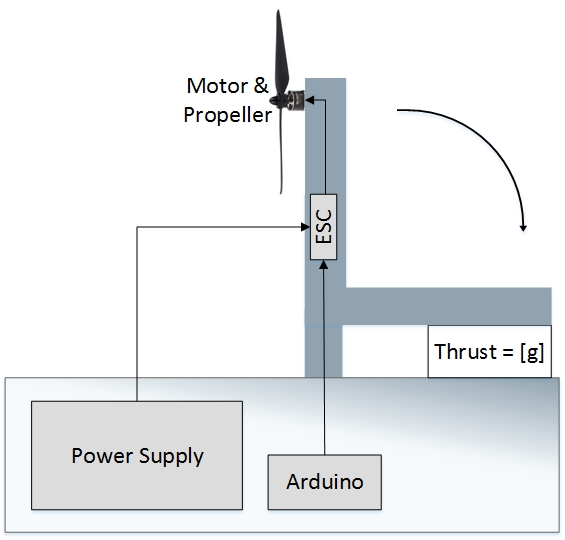
\includegraphics[width = 0.6\textwidth]{VAPIQ-PICTURES/TestSetup5}
    \caption{Test Setup: Motor Propeller Thrust Test Rig}
    \label{fig:TestSetup5}
\end{figure}
\noindent In this test a potentiometer was used to adjust thrust. The potentiometer values are mapped to values between 1000 and 2000 microseconds. Both motors were tested for several PWM values and the respective thrust values were noted.\\
\\
In Appendix A9 the code used for TR005 can be found. 

\subsubsection*{\textsc{\medium Test Assessment}}
% [Enter a comprehensive assessment of your interpretation of how adequate the test was in light of how thorough the test plan said it should be? What wasn't tested well enough?]
The test rig gives a good indication of the actual thrust produced by the motor propeller combinations. The rig may have some measuring inaccuracies due to the small variations in mechanical mounting, the difference in width of the mounting plate in comparison with the real quadcopter arm and the calibration of the weight.

\subsubsection*{\textsc{\medium Test Results}}
For our purposes, these tests have yielded the results needed in order to evaluate the performance of the motors and propellers.\\
\\
In Fig. \ref{fig:fpq3} and \ref{fig:fpq1} the result from this test is displayed. 
\begin{figure}[H]
    \centering
    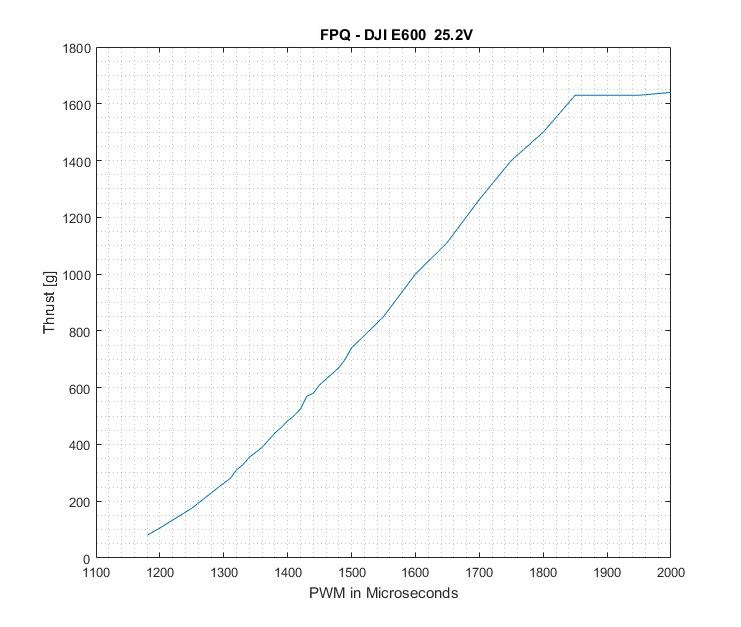
\includegraphics[width = 0.6\textwidth]{VAPIQ-PICTURES/FPQ3}
    \caption{DJI E600with PS 25.2V: Motor Propeller Thrust Test Rig}
    \label{fig:fpq3}
\end{figure}

\begin{figure}[H]
    \centering
    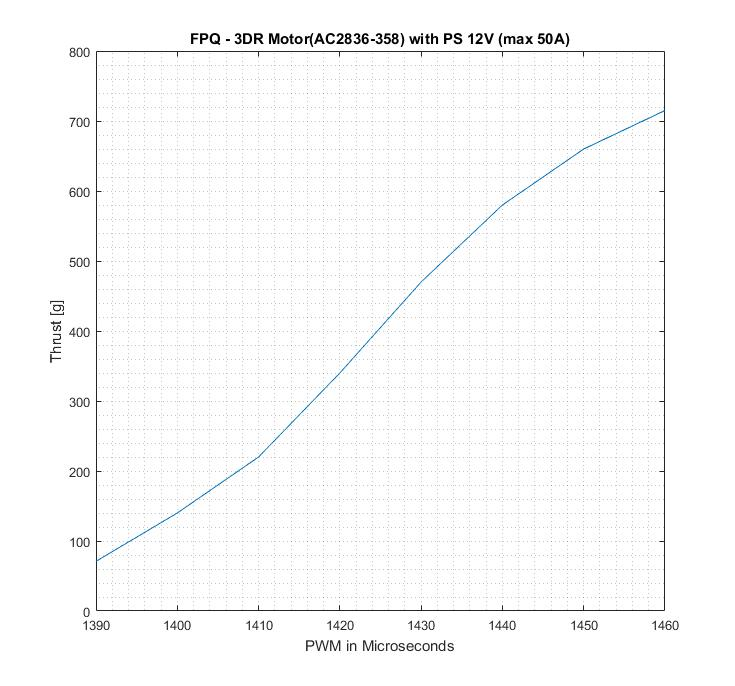
\includegraphics[width = 0.6\textwidth]{VAPIQ-PICTURES/FPQ1}
    \caption{3DR Motor(AC2836-358) with PS 12V: Motor Propeller Thrust Test Rig}
    \label{fig:fpq1}
\end{figure}

\noindent
Full test result matrix for TR005 can be found in Appendix B1.
 
 
\newpage       
%%%%%%%%%%%%%%%%%%%%%%%%%%%%%%%%%%%%%%
\subsection{TR007: Variable Pitch Test - g/W and Servo Angle Input}
\tr{T015}{AC018}{5}{BL048}{VPQ-126}
         {\shortstack[l]{GIVEN that we have mounted a variable pitch mechanism to the thrust \\ test rig, WHEN we adjust the pitch and/or thrust, THEN the respective\\ thrust in grams shall be displayed on weight.}}


\subsubsection*{\textsc{\medium Purpose}}
The purpose of TR007 is to evaluate the efficiency of the variable pitch assembly as well as to provide information about the most efficient pitch angle. 

\subsubsection*{\textsc{\medium Test Setup}}
In Tab. \ref{tab:tabt8} and \ref{tab:tabt9} the equipment used conducting TR007 is displayed. 
\begin {table}[H]
    \begin{center}
    \caption {Test Equipment: Variable Pitch Test } 
    \label{tab:tabt8} 
    \begin{tabular}{|l|}\hline 
        Power SupplyEA-PS 2342-06 B           \\ \hline
        Microcontoller Arduino Nano ATmega328P \\ \hline
        Motor \\ \hline
        ESC\\ \hline    
        \end{tabular}
    \end{center}
\end{table}

\begin {table}[H]
    \begin{center}
    \caption {Motor Propeller Combination: Variable Pitch Test} 
    \label{tab:tabt9} 
    \begin{tabular}{|l|l|}\hline 
        Motor Test No. 1: & Motor Test No. 2:  \\ \hline
        3DR AC2836-358  & AXI 2208/26 \\ \hline
        Align mechanism with 9" propeller & Model Motors mechanism with 8" propeller \\ \hline
        3DR 20A-BEC & Multistar 12A - Turnigy \\ \hline
        880KV & 1420KV \\ \hline
        \end{tabular}
    \end{center}
\end{table}
\newpage
\noindent In Fig. \ref{fig:VPM} the test setup for TR007 is displayed.
\begin{figure}[H]
    \centering
    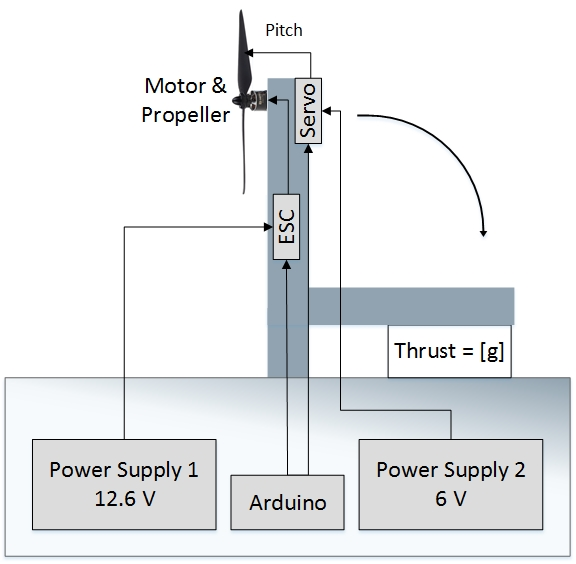
\includegraphics[width = 0.6\textwidth]{VAPIQ-PICTURES/TestSetup7}
    \caption{Test Setup: Variable Pitch Test}
    \label{fig:VPM}
\end{figure}
\noindent
In this test a servo was mounted to the Thrust Test Rig as shown in Fig. \ref{fig:VPM}. The servo adjusts the pitch angle on the variable pitch mechanism. In this test two potentiometers are used; one to adjust thrust and another to adjust the pitch angle. The potentiometer values are mapped to thrust values between 1000 and 2000 microseconds. The potentiometer for the pitch angle is mapped to have the same value as the servo angle input.\\
\\
In Appendix A9 the code used for TR007 can be found. 


\subsubsection*{\textsc{\medium Test Assessment}}
% [Enter a comprehensive assessment of your interpretation of how adequate the test was in light of how thorough the test plan said it should be? What wasn't tested well enough?]
%[Describe any variances between the testing that was planned and the testing that actually occurred.  Also, provide an assessment of the manner in which the test environment may be different from the operational environment and the effect of this difference on the test results
%[Provide a brief description of the unexpected results, problems, or defects that occurred during the testing.]
The test rig gives a good indication of the actual thrust produced by the motor propeller combinations. The rig may have some measuring inaccuracies due to the small variations in mechanical mounting, the difference in width of the mounting plate in comparison with a real quadcopter arm and the calibration of the weight.\\
\\
The servo value input for both the tests are not the same. The reason for this is that the test with the 3DR motor and Align mechanism needed a stronger servo motor. The servo motors were not mounted and configured in the same way.\\
\\
When a stronger servo was mounted to the 3DR motor and Align mechanism; it was still not strong enough to hold the pitch mechanism in place. \\
\\

\newpage
\subsubsection*{\textsc{\medium Test Results}}
In Fig. \ref{fig:vpm1} and \ref{fig:vpm2} the result from this test is displayed. 
\begin{figure}[H]
    \centering
    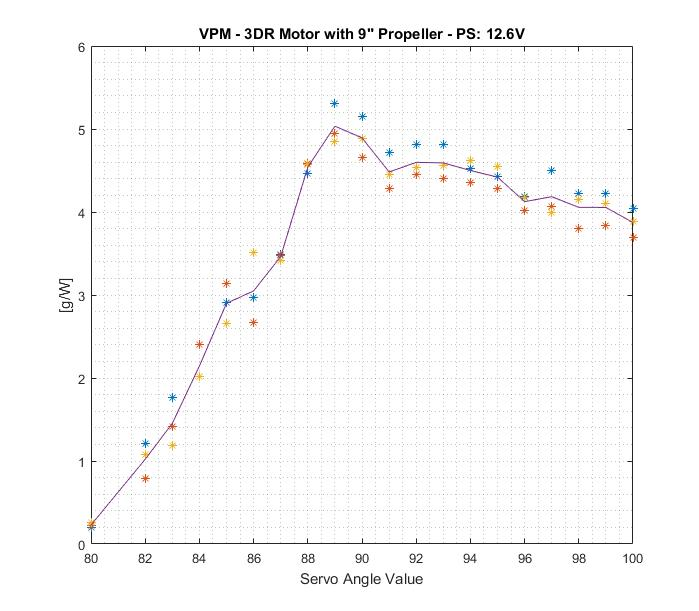
\includegraphics[width = 0.65\textwidth]{VAPIQ-PICTURES/VPM1}
    \caption{3DR Motor Efficiency: Variable Pitch Test}
    \label{fig:vpm1}
\end{figure}
\begin{figure}[H]
    \centering
    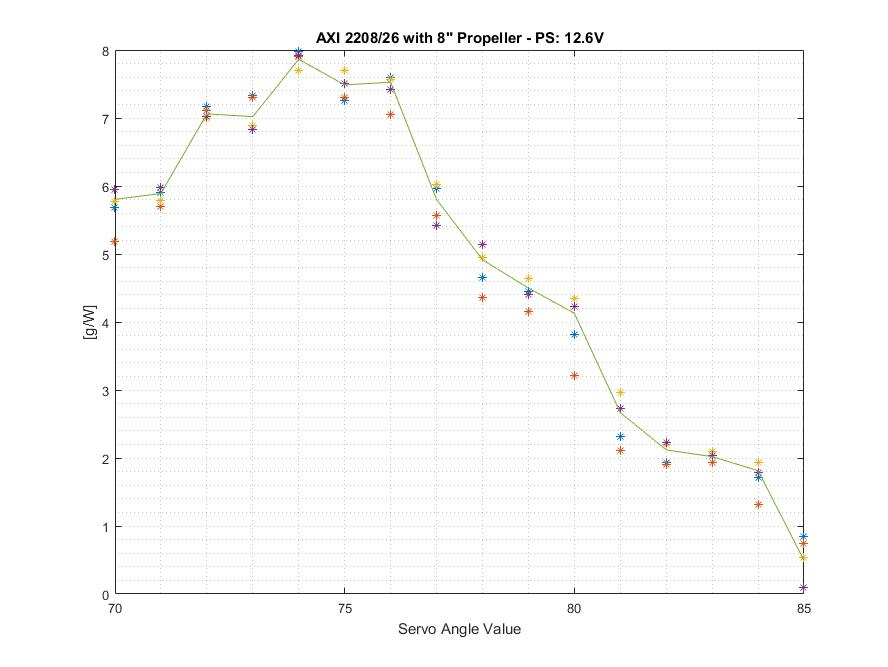
\includegraphics[width = 0.65\textwidth]{VAPIQ-PICTURES/VPM2}
    \caption{AXI Motor Efficiency: Variable Pitch Test}
    \label{fig:vpm2}
\end{figure}

\noindent
In Fig.\ref{fig:vpm1} it can be seen that the maximum efficiency for the 3DR motor and Align mechanism is when the servo angle value is at 89. This servo angle value is approximated to be about 7 degrees on the pitch mechanism. It also needs to be stated that the servos used in this particular test were not strong enough. The servo motor was not able to keep the desired pitch angle during the test. \\
\\
In Fig.\ref{fig:vpm2} it can be seen that the maximum efficiency for the AXI motor and Motor Model mechanism is when the servo angle value is around 74. This servo angle value is approximated to be around 6 degrees on the pitch mechanism.\\
\\
Full test result matrix for TR007 can be found in Appendix B2.
\newpage